\section{Test}
\subsection{Privacy and Security}
\subsubsection{Privacy Issues}
The only data about a \textbf{User} stored and managed by the application is just the one submitted by the \textbf{User} himself at login time, plus a timestamp of the last login.\\
The only data about a \textbf{User} visible by other \textbf{Users} are: \textit{username}, \textit{country}, \textit{team name}, \textit{points}. \\
The timestamp of the last login is used for applicative purposes only, and it’s aggregated in evaluating the \textbf{Analytics}. For no reason \textit{admins} or other \textbf{Users} can access to the last login timestamp of a \textbf{User}.
\subsubsection{Password Encryption}
As discussed in the paragraph 4.3.3, all the \textbf{Users}’ passwords are strongly encrypted and they are never compared using their plain text version. \\
The encryption is performed immediately after the click on the submit button, this means that no module/class/driver/DB of the application can have access to the plain text password, but the Password Encryptor itself.\\
Moreover, given the encrypted password, there is no way to retrieve back the plain text one, nor to correctly access to the application using the hashed one.\\
The application does not deal with Record \& Playback attacks, anyway having no access to the source Java code is very difficult to use it to successfully steal an account.
\subsubsection{Input Injections}
\textbf{N.B.} In the real implementation we used an input obfuscation to hide password input. In the following example it has been removed for demonstrative purposes only.

\begin{figure}[H]
	\centering
	\caption{Example 1: : \textit{usernames} are real registered \textit{username}, \textit{passwords} are famous MongoDB injection strings.}
	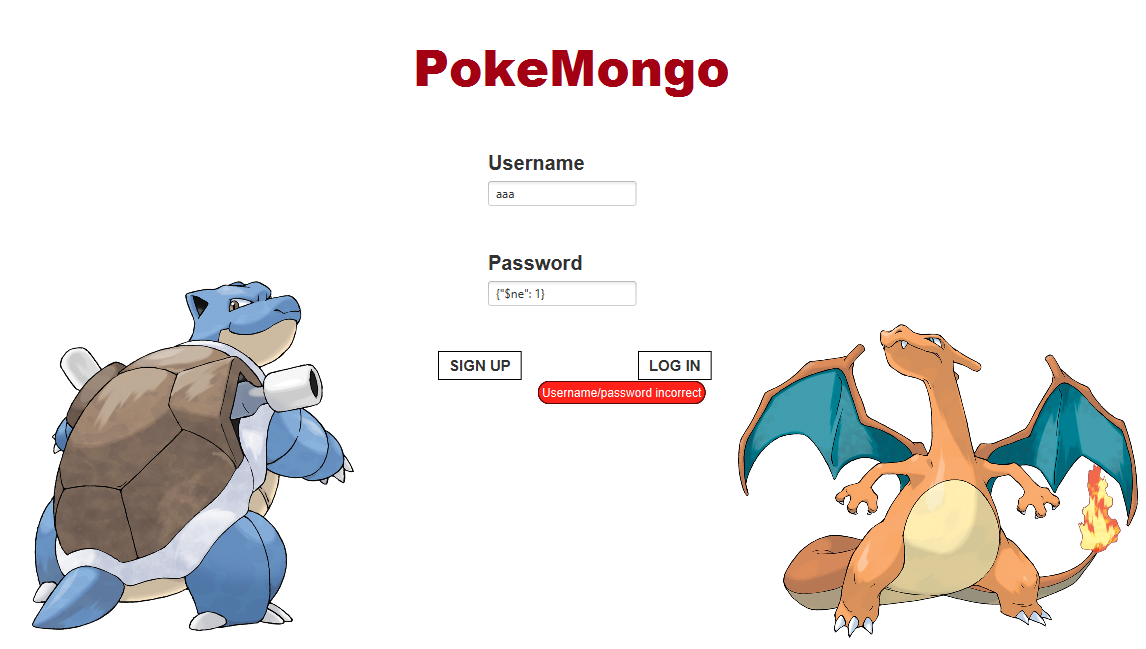
\includegraphics[width=\textwidth]{img/privacy_1.png}
\end{figure}
\begin{figure}[H]
	\centering
	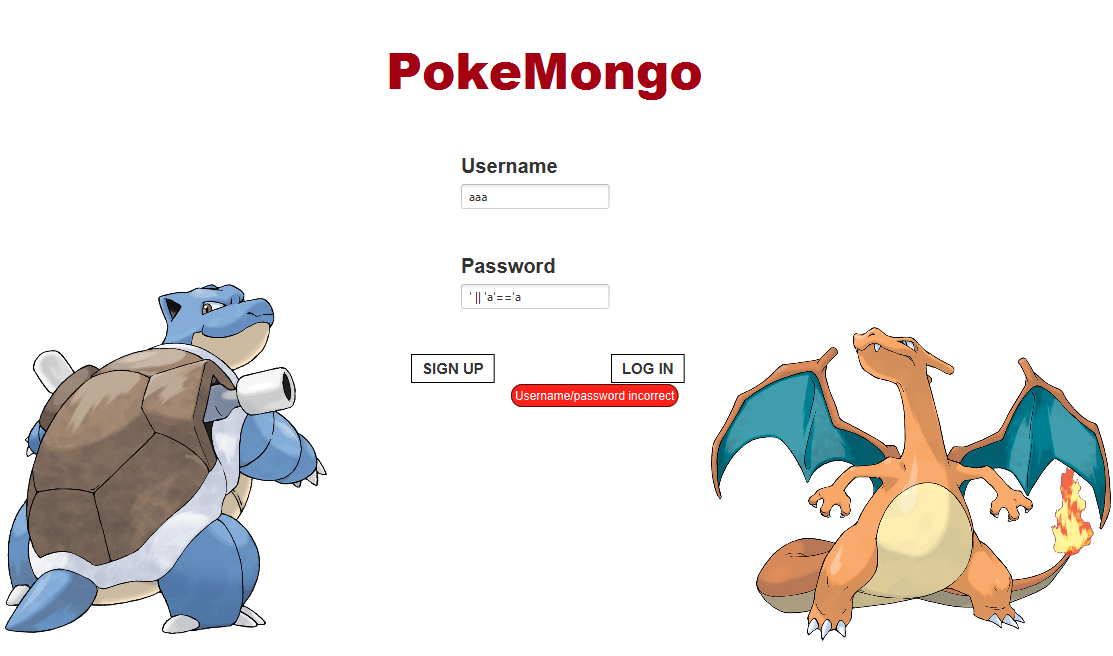
\includegraphics[width=\textwidth]{img/privacy_2.png}
\end{figure}


\begin{figure}[H]
	\centering
	\caption{Example 2: input validation on the signup form blocks code injection attempts (it would have removed all the collection)}
	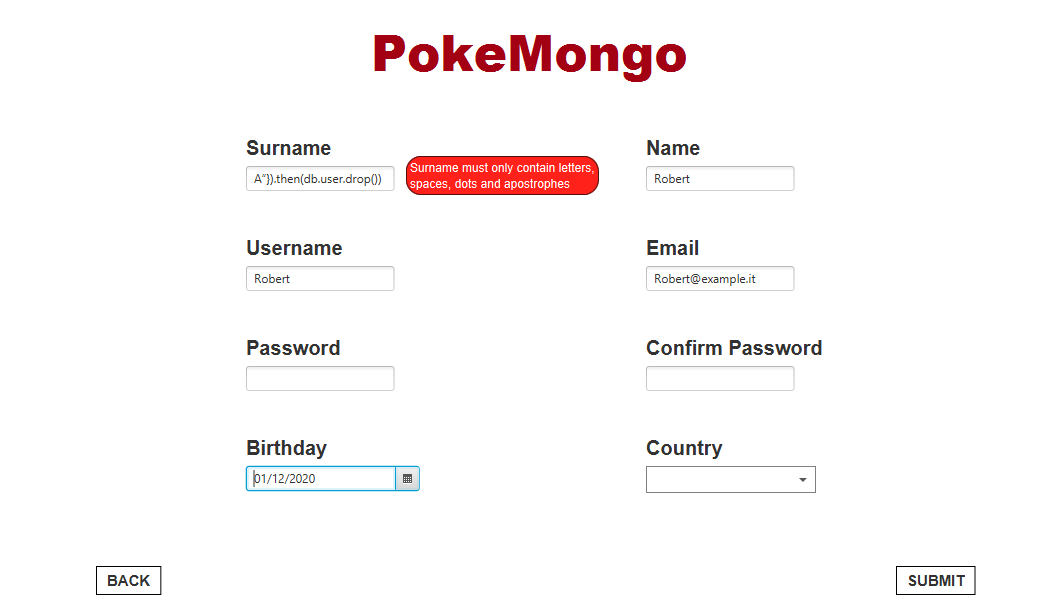
\includegraphics[width=\textwidth]{img/privacy_3.png}
\end{figure}


\subsection{Unit Test}
While writing the implementation of the various Classes of the project, Unit Tests were written in order to check if the modules were working properly. The main types of test written are the following:
\begin{itemize}
	\item \textbf{Singleton Check}: whenever a Singleton Pattern is implemented in a class there is a test that will check if two instance of the same class are the same. Here are some examples of these tests:
\begin{lstlisting}[language=Java]
//Cache
public void WHEN_getInstance_invoked_twice_THEN_same_ instance_returned(){
	PokeMongoImageCache pkic2 = PokeMongoImageCache.getInstance();
	Assertions.assertEquals(pkic, pkic2);
}
\end{lstlisting}
	\item \textbf{Exception Check}: in many parts of the code there will be tested if a particular input will generate or not an Exception (both cases are present). Here are some examples of these tests:
\begin{lstlisting}[language=Java]
//PokemonManagerOnMongoDb
public void WHEN_insert_invoked_with_non_Pokemon_
parameter_THEN_Exception_not_thrown(){
	Assertions.assertDoesNotThrow( ()->{
		PokemonManagerOnMongoDb pokemonManagerOnMongoDb = new PokemonManagerOnMongoDb();
		Object c = new Character('c');
		pokemonManagerOnMongoDb.insert(c);
	});
}
public void WHEN_update_invoked_with_non_Bson_parameter_
newvalue_THEN_Exception_not_thrown(){
	Assertions.assertDoesNotThrow( ()->{
		PokemonManagerOnMongoDb pokemonManagerOnMongoDb = new PokemonManagerOnMongoDb();
		Object c = new Character('c');
		pokemonManagerOnMongoDb.getWithFilter(c);
	});
}

//TeamManagerOnNeo4j NOTE THE "KISS" TEST
public void WHEN_getPokemons_invoked_with_non_
ArrayOfRecords_parameter_THEN_ClassCastException_thrown(){
	Assertions.assertThrows(ClassCastException.class, ()->{
		TeamManagerOnNeo4j teamManagerOnNeo4j = new TeamManagerOnNeo4j();
		
		Object c = new Character('c');
		ArrayList<Object> cList = new ArrayList<>();
		cList.add(c);
		ArrayList<Pokemon> arrayList = new ArrayList<Pokemon>();
		teamManagerOnNeo4j.getPokemons(arrayList, cList);
	});
}
\end{lstlisting}
	
	\item \textbf{Bad Input Check}: general check that a "bad input" (like an empty string, a NaN ...) in some particular classes will generate the predicted response. These tests are particularly performed in the \textbf{Form Validator}. Here are some examples of these tests:
\begin{lstlisting}[language=Java]
//FormValidatorPokeMongo
public void WHEN_isPersonNoun_invoked_with_empty_
string_THEN_false_returned(){
	Assertions.assertFalse(formValidatorPokeMongo.isPersonNoun(""));
}

public void WHEN_isValidEmail_invoked_with_empty_
string_THEN_false_returned(){
	Assertions.assertFalse(formValidatorPokeMongo.isValidEmail(""));
}

public void WHEN_isValidPassword_invoked_with_empty_
string_THEN_false_returned(){
	Assertions.assertFalse(formValidatorPokeMongo.isValidPassword(""));
}

\end{lstlisting} 
	\item \textbf{Security Check}: check of the goodness of the \textbf {Security} class in terms functionality with bad inputs, same output check with same input and so on. Here are some examples of these tests:
\begin{lstlisting}[language=Java]
//PasswordEncryptor
public void WHEN_encrypt_password_invoked_twice_
with_same_input_THEN_same_output_returned(){
	String out1 = PasswordEncryptor.encryptPassword("prova1");
	String out2 = PasswordEncryptor.encryptPassword("prova1");
	Assertions.assertEquals(out1, out2);
}

public void WHEN_encrypt_password_invoked_twice_
with_different_input_THEN_different_output_returned(){
	String out1 = PasswordEncryptor.encryptPassword("prova1");
	String out2 = PasswordEncryptor.encryptPassword("prova2");
	Assertions.assertNotEquals(out1, out2);
}

public void WHEN_encrypt_password_invoked_with_empty_
string_THEN_non_empty_output_returned(){
	String out = PasswordEncryptor.encryptPassword("");
	Assertions.assertNotEquals(out, "");
}
\end{lstlisting}
\end{itemize}
\subsection{Robustness}
\subsection{Performance}
